\documentclass[preprint]{/Users/jesse/tex/aastex_JRF}

\usepackage{graphicx}
\usepackage[space]{grffile}
\usepackage{latexsym}
\usepackage{amsfonts,amsmath,amssymb}
\usepackage{url}
\usepackage[utf8]{inputenc}
\usepackage{fancyref}
\usepackage{hyperref}
\hypersetup{colorlinks=false,pdfborder={0 0 0},}
\usepackage{textcomp}
\usepackage{longtable}
\usepackage{multirow,booktabs}



\begin{document}

\title{Deep Pulsar Searches in Ultra-Faint Dwarf Galaxies}
\author{Jesse Feddersen\\ \emph{Department of Astronomy, Yale University}\\~\\}

\maketitle 

%\begin{figure}[h!]
%\begin{center}
%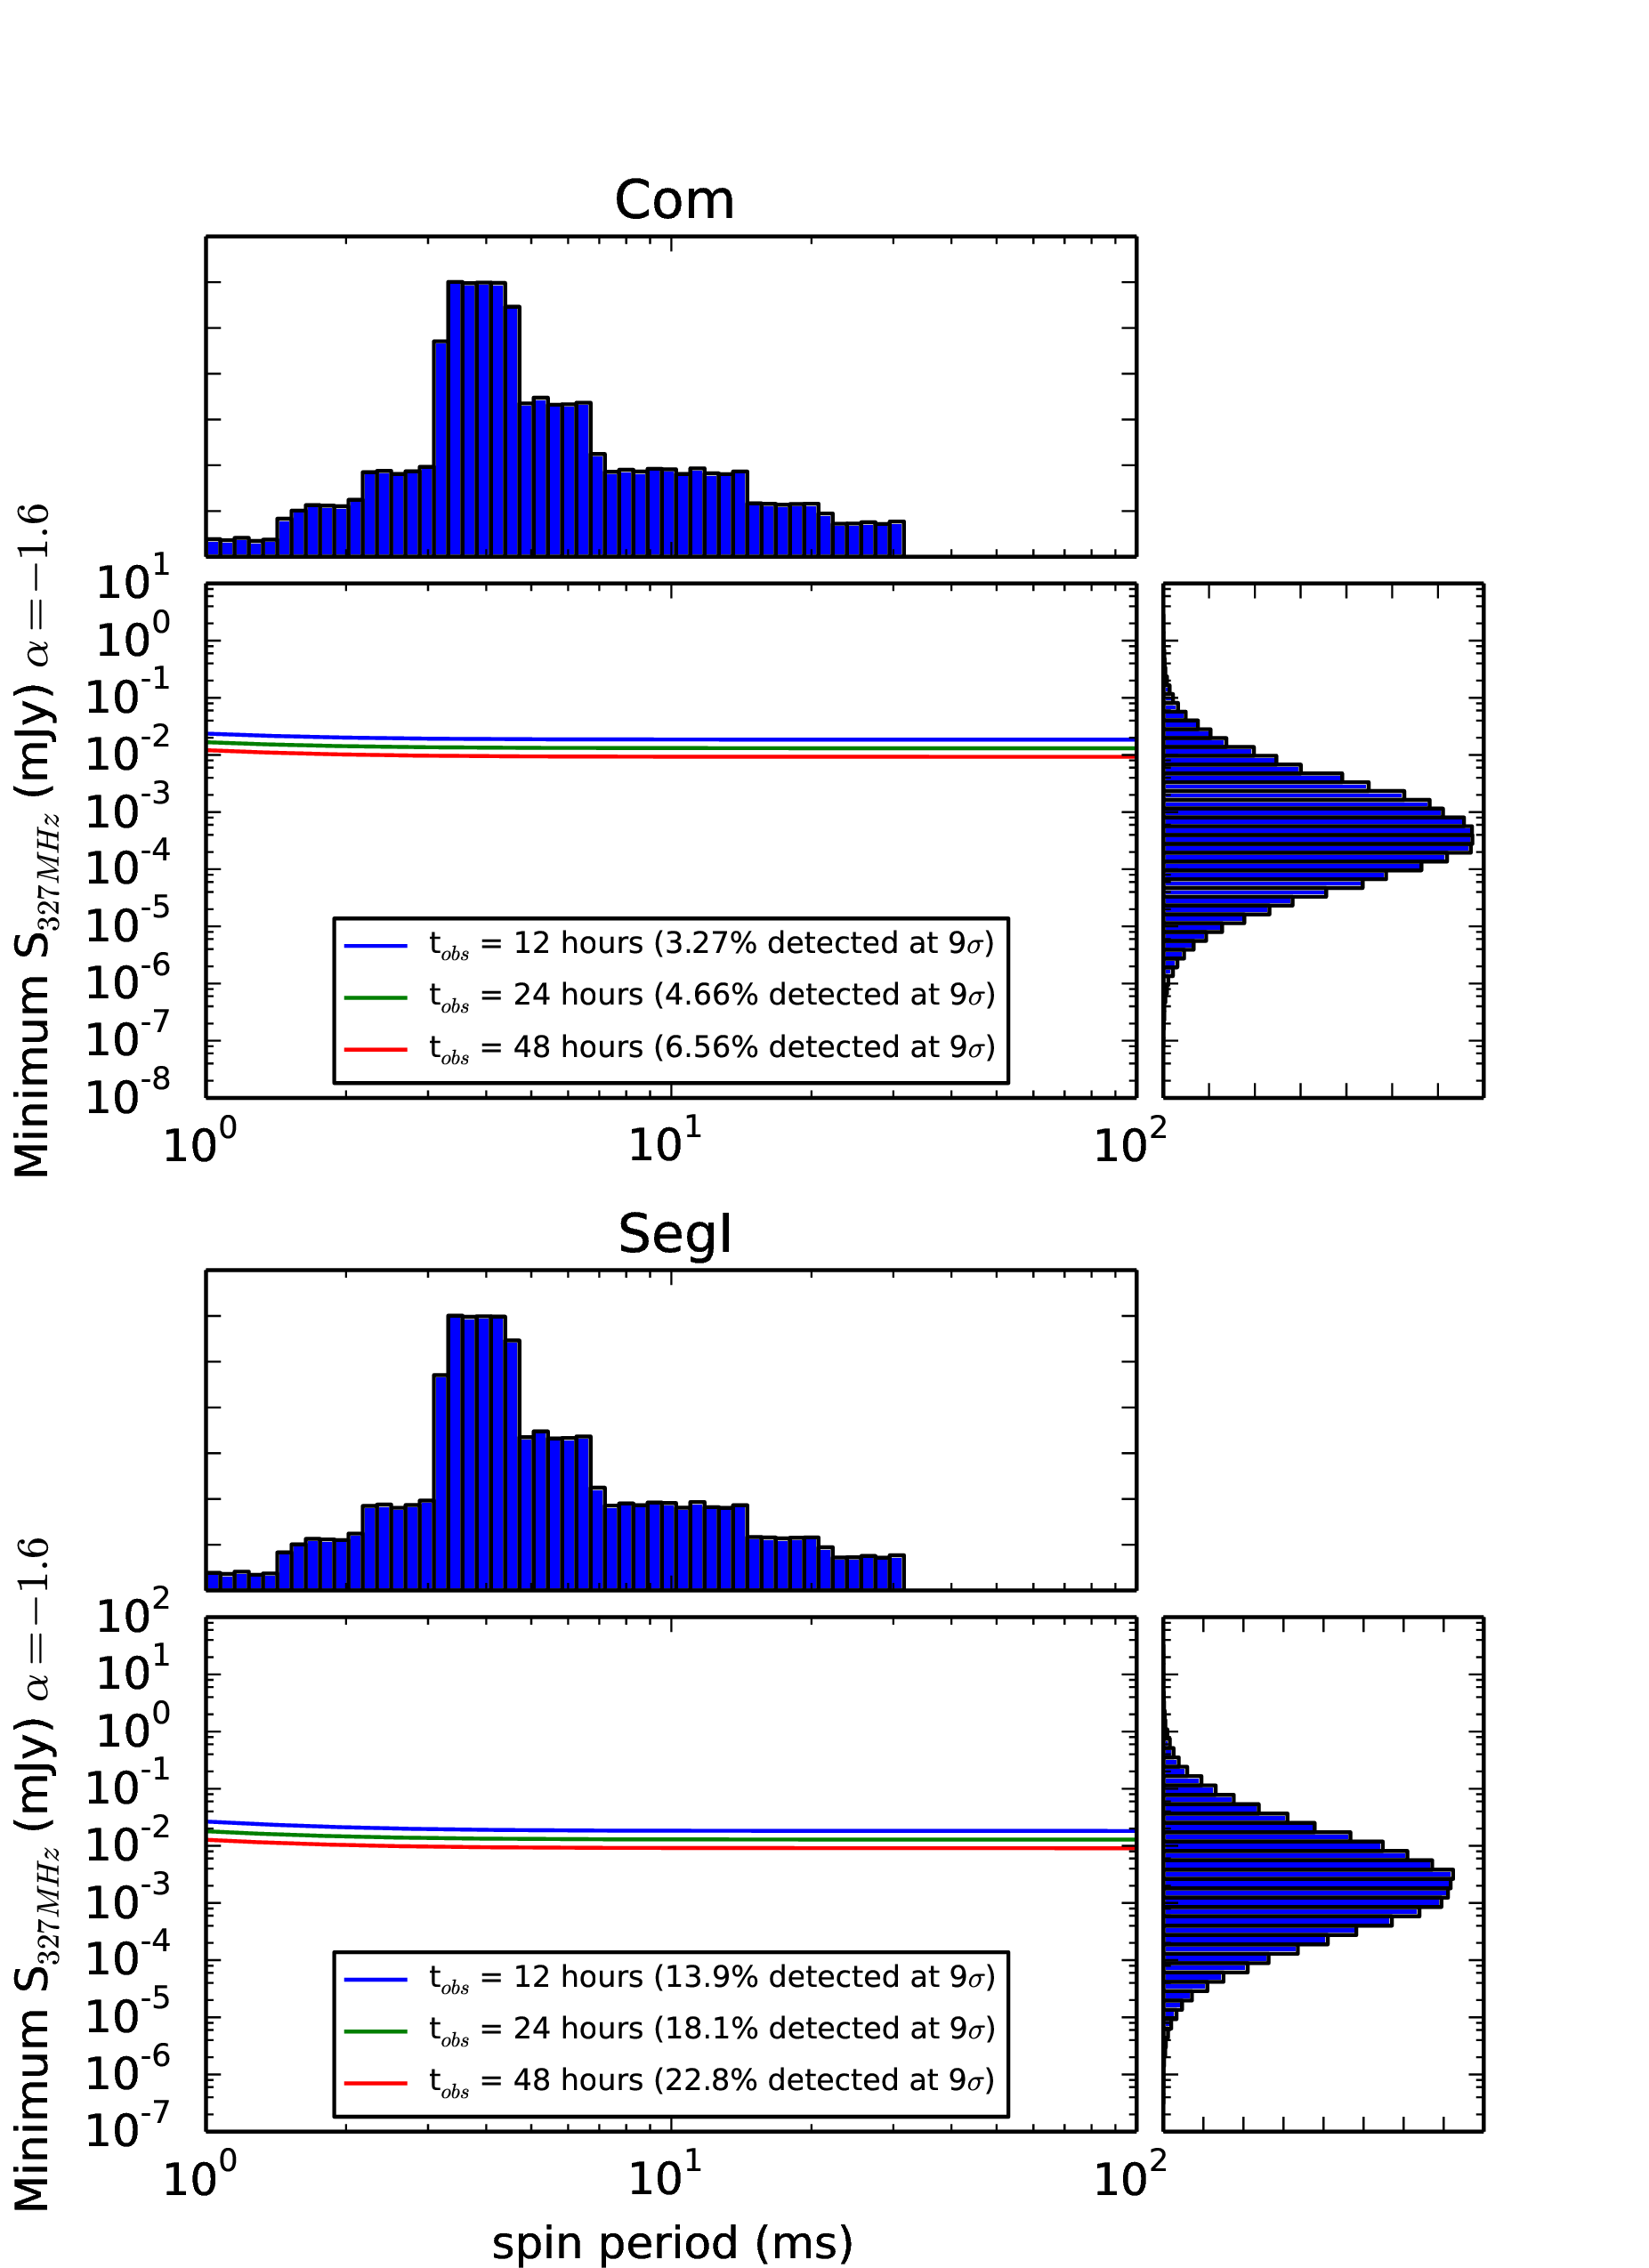
\includegraphics[width=0.98\columnwidth]{figures/knownmsps/327PUPPI_sensitivity.png}
%\caption{Replace this text with your caption}
%\end{center}
%\end{figure}
%
Our search for pulsars in ultra-faint dwarf galaxies will address three main science goals:
\begin{enumerate}
\item The discovery or a pulsar in a UFD would be the \textbf{first known extragalactic pulsar outside of the Magellanic Clouds}.
\item Placing observational limits on the pulsar population in UFDs will provide the first \textbf{constraint on the high-mass initial mass function} (IMF) of the oldest dynamically unevolved stellar populations.
\item By measuring the dispersion of the pulses from a pulsar in a UFD, we \textbf{probe the electron density of the intergalactic medium} towards that line of sight.
\end{enumerate}
We justify each of these goals in turn.

\section{First of its Kind}
%Put a short history of pulsar surveys here. March to farther distances. 
%Summarize the pulsar population, disk, GCs, Magellanic Clouds, link to expected properties of UFD pulsar (MSP)


\section{Constraining the High-Mass IMF}
%Short history of IMF, recent evidence of variation, Marla's work on low-mass IMF (bottom-light) in UFDs. Distribution of neutron stars from different IMF forms.
The initial mass function is the distribution of stellar masses in a stellar population at the beginning of star formation. The IMF determines the evolution of the population and is a crucial input in models of synthetic stellar populations. The form of the IMF affects many galaxy parameters derived from stellar population synthesis. The form of the IMF also places a constraint on star formation theory, which must predict the observed IMF. In the Milky Way, the IMF is typically parametrized by the similar~\citet{Kroupa01} or~\citet{Chabrier03} laws with little variation across a range of star-forming environments~\citep{Bastian10}. A departure from this ``universal'' IMF indicates  a star formation process that depends on environment.



\section{Probing the Intergalactic Medium}
%dispersion measure. 

\bibliographystyle{/Users/jesse/tex/astronat/apj/apj.bst} 
\bibliography{/Users/jesse/tex/astronat/apj/apj-jour.bib,/Users/jesse/Dropbox/all.bib}

\end{document}

